% !TEX root = marvin.tex
\begin{figure*}[t]
  \begin{center}
  \iflatexml
  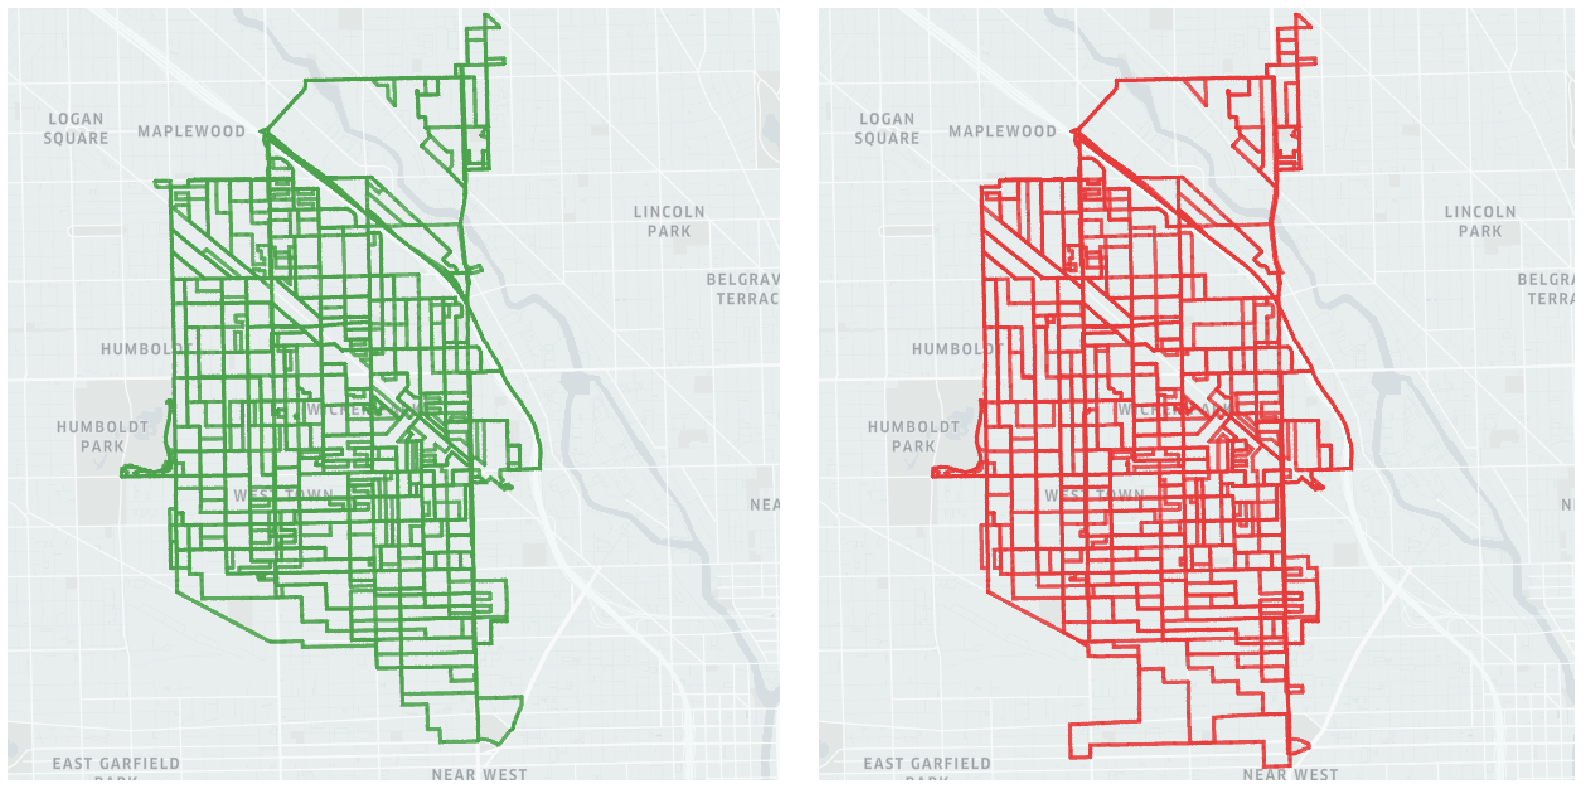
\includegraphics[width=6\textwidth]{figs/vin_gvin_all.png}
  \else
    \begin{tabular}{ll}
      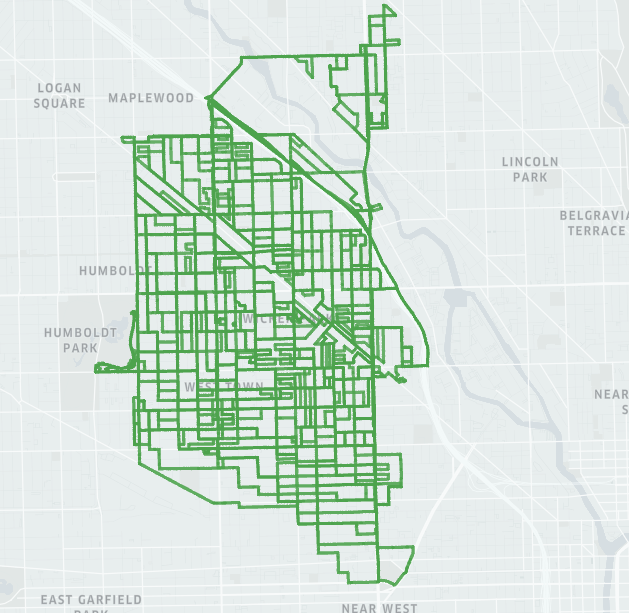
\includegraphics[height=8.1cm,trim={0.2cm 0 0.4cm 0},clip]{figs/vin_gvin_vin.png} &
      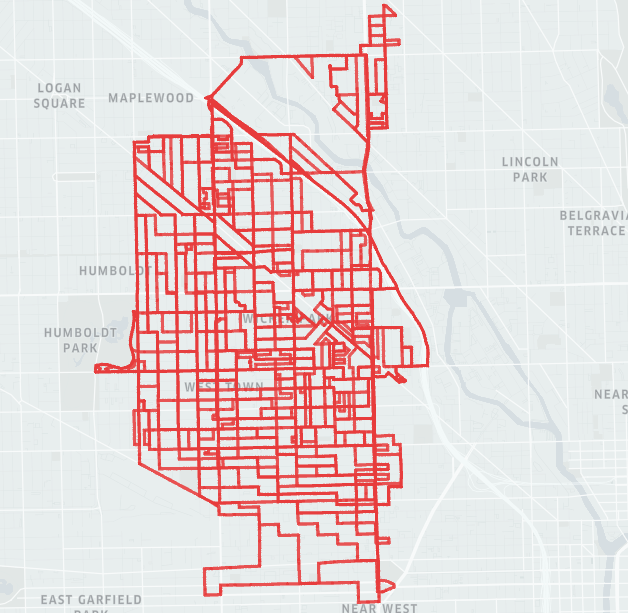
\includegraphics[height=8.1cm,trim={0.2cm 0 0.8cm 0},clip]{figs/vin_gvin_gvin.png} \\
    \end{tabular}
  \fi
  % \vspace{-0.15in}
  \caption{Bird's eye view of a partially complete traversal
  of MARVIN (left) and of the GVIN (right). While slightly more
  spread out, the traversal of the GVIN leaves many small streets
  unvisited and is less thorough overall.}
  \label{fig:vin_gvin}
  \end{center}
\end{figure*}